\section{Introduction}\label{sec:intro}

World-model-augmented robot policies predict future images, latent observation
features, or visual subgoals and supply them to an action generator
\citep{vpp2024,susie2024,dreamvla2025,worldvla2025,ahead2026,futurevla2026,lawam2026}.
This design is appealing because a predicted future can summarize how the
scene should change without decoding a video at deployment.  Yet future-state
accuracy is not a control result.  World-model quality correlates only weakly
with planning performance in WorldArena \citep{worldarena2026}, and auxiliary
prediction can change a shared representation even when the controller ignores
the predicted content.  A system-level benchmark gain therefore does not show
that the future representation caused the gain.

A future condition has two semantics: \emph{what} state is predicted and
\emph{when} that state should occur.  This distinction matters for policies
that generate an action chunk and execute only a prefix before replanning.  A
target at the chunk endpoint can directly specify the state to be reached by
the current proposal.  A milestone several chunks away can still be useful,
but it behaves as a high-level subgoal unless the policy also knows its horizon
or converts it into a local target.  Most evaluations conflate this temporal
contract with predictor quality, conditioning capacity, auxiliary gradients,
and policy initialization.

We study these factors through three interfaces (Fig.~\ref{fig:overview}).
The released LaWAM system predicts a future visual grid and cross-attends to it
inside a flow-matching action expert \citep{lawam2026}.  MINT-VLA recomputes a
recurrence-defined milestone in the trainable policy encoder and injects one
predicted prefix token.  Our \emph{PredictiveActionAdapter} instead predicts a
future patch-grid residual from the current visual tokens and each flow action
proposal, then returns a zero-initialized correction to the corresponding
action-expert tokens.  These systems differ in target horizon and conditioning
location, but no architectural difference is interpreted causally without its
own intervention.

\begin{figure}[t]
  \centering
  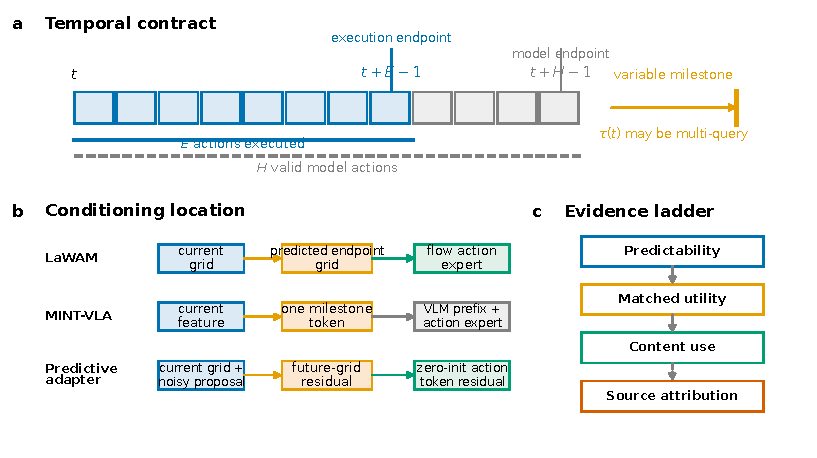
\includegraphics{figures/fig1_contract.pdf}
  \caption{\textbf{Temporal contracts, conditioning interfaces, and evidence
  levels.} \textbf{a}, A VLA predicts $H$ valid actions and executes $E\leq H$
  before replanning.  A target at $\tau(t)$ may coincide with either endpoint
  or lie several queries ahead. \textbf{b}, The evaluated interfaces place a
  predicted future grid in LaWAM's action-expert context, a pooled milestone
  token in the $\pi_{0.5}$ prefix, or a proposal-conditioned residual directly
  on $\pi_{0.5}$ action tokens. \textbf{c}, Prediction, matched utility,
  content use, and source attribution require separate evidence; an arrow
  denotes a required progression, not a logical implication.}
  \label{fig:overview}
\end{figure}

The resulting evidence is asymmetric.  A CPU source audit finds that the
released LaWAM RoboTwin condition is aligned with its 36-action execution
endpoint.  At that frozen checkpoint, normal prediction reaches 94.00\%
success, versus 40.33\% when future content is replaced by a deterministic
within-task, different-episode shuffle.  The +53.67-point paired difference has
a hierarchical 95\% interval of [$+36.08$,$+68.58$], and every task and
evaluation seed is positive.  Null and persistence controls also pass.  Thus
the released policy uses the specific predicted endpoint content in closed
loop.  This fixed-checkpoint intervention does not determine whether the
dependence was created by LaWAM pretraining, downstream auxiliary shaping, or
inference-time conditioning.

The negative cases show why each evidentiary step is necessary.  MINT-VLA
predicts held-out milestones better than persistence but is 8.58 points below
matched no-hint training across three seeds.  PredictiveActionAdapter adds only
0.50\% parameters and passes an offline action-conditioning test, but its
apparent +11.61-point effect against one fixed A0 becomes +1.94 points with a
95\% interval of [$-5.78$,$+12.75$] after independently training all three A0
seeds.  It also contains task regressions and no resolved normal--shuffled
effect.  Finally, changing the executed prefix from 36 to 50 actions does not
produce a local-world-model-specific cadence effect.  Temporal alignment is
therefore a measured distinction and a plausible design hypothesis, not an
established explanation of these outcomes.

This paper makes three contributions:
\begin{itemize}
  \item We formalize the temporal contract between a predicted target, a VLA
  action horizon, and its executed prefix, and define an evidence ladder that
  prevents representation quality or public-system scores from standing in
  for control causality.
  \item We introduce two controlled milestone interfaces, including a
  policy-preserving PredictiveActionAdapter that maps each noisy flow proposal
  to a future-grid residual and an action-indexed correction while retaining
  exact base behavior at initialization.
  \item We provide paired content interventions, independently matched training
  seeds, and task-level safety analyses that establish strong future-content
  use in one released LaWAM checkpoint while rejecting broader utility claims
  for the evaluated MINT-VLA and predictive-adapter instances.
\end{itemize}
